\documentclass[11pt, aspectratio = 169]{beamer}
% \documentclass[12pt]{article}
% \usepackage{beamerarticle}

% \usetheme{Dresden} % Alternatively: Darmstadt, Madrid, Warsaw, ...
% \useoutertheme{miniframes} % Alternatively: miniframes, infolines, split
% \useinnertheme{rounded}
% \usecolortheme{beaver} % Alternatively: albatross, beaver, crane, ...
\usefonttheme{default}  % Alternatively: serif, structurebold, ...
\renewcommand\mathfamilydefault{\rmdefault}
\setbeamerfont{subtitle}{size = \small}
\setbeamercovered{transparent}
\setbeamertemplate{navigation symbols}{}
\setbeamertemplate{caption}[numbered]
\setbeamertemplate{title page}[empty]
\setbeamertemplate{footline}[frame number]

\definecolor{clemsonpurple}{HTML}{522D80}
\definecolor{clemsonorange}{HTML}{F66733}

\setbeamercolor{frametitle}{fg = clemsonpurple, bg = white}
\setbeamercolor{title}{fg = clemsonpurple, bg = white}
\setbeamercolor{local structure}{fg = clemsonpurple}
\setbeamercolor{block title}{fg = clemsonpurple}
\setbeamercolor{section in toc}{fg = clemsonpurple, bg = white}
\setbeamercolor{subsection in toc}{fg = clemsonorange, bg = white}
\setbeamercolor{footline}{fg = clemsonpurple!50, bg = white}
\setbeamercolor{item projected}{fg = clemsonpurple, bg = white}
\setbeamercolor{alerted text}{fg = clemsonorange, bg = white}
\setbeamertemplate{itemize item}{\color{clemsonpurple}$\bullet$}
\setbeamertemplate{itemize subitem}{\color{clemsonpurple}\scriptsize{$\bullet$}}
\let\Tiny=\tiny

\AtBeginPart{}
\AtBeginSection{}
\AtBeginSubsection{}
\AtBeginSubsubsection{}
\setlength{\emergencystretch}{0em} % Prevent overfull lines
\setlength{\parskip}{0pt}

% \usepackage{fontspec}
% \setsansfont{Myriad Pro}
% \setmonofont{Consolas}

\usepackage[scale=0.95]{noto-sans}
\usepackage[scale=0.95]{noto-mono}
\usepackage[T1]{fontenc}
\usepackage{amsmath}
\usepackage{microtype}
\usepackage{graphicx}

\usepackage{tikz}
\usetikzlibrary{positioning}

\usepackage{listings}
\lstset{
    basicstyle = \footnotesize\ttfamily,
    columns = fullflexible,
    keepspaces = true,
    numbers = left,
    breaklines = true,
    breakatwhitespace = true,
    frame = single,
    % aboveskip = \bigskipamount,
    % belowskip = \bigskipamount,
    xleftmargin = \parindent,
    xrightmargin = \parindent,
}

\newcommand{\indep}{\perp \!\!\! \perp}

\title[]{Statistical Methods in Survival Analysis}
\author[]{Zhen-Huan (Kenny) Hu, MPH}

\institute[CIBMTR]{Center for International Blood and Marrow Transplant Research\\Medical College of Wisconsin}

\begin{document}

\begin{frame}[plain]
  \titlepage
\end{frame}


\begin{frame}
  \frametitle{Outline}
  \tableofcontents
\end{frame}

\section{Basic functions}

\begin{frame}
  \frametitle{Survival function}
  \textbf{Survival function} Probability of a subject experiencing the event after time $t$:
  \begin{equation*}
    S(t) = P(T > t)
  \end{equation*}
  where $T$ denotes the time to event (which is a random variable).
  
  \textbf{Failure function} Probability of a subject experiencing the event before or at time $t$ (complement of $S(t)$ and CDF of time to event $T$):
  \begin{equation*}
    F(t) = P(T \le t) = 1 - S(t)
  \end{equation*}
  \begin{equation*}
    S(t) = 1 - F(t)
  \end{equation*}

  \textbf{Event rate} at time $t$ (PDF of time to event $T$):
  \begin{equation*}
    f(t) = \lim_{\Delta t \to 0} \frac{P(t \le T < t + \Delta t)}{\Delta t} = \frac{d}{dt}F(t) = - \frac{d}{dt}S(t)
  \end{equation*}
  \begin{equation*}
    F(t) = \int_{0}^{t}f(u)du
    \quad
    S(t) = \int_{t}^{\infty}f(u)du
  \end{equation*}
\end{frame}

\begin{frame}
  \frametitle{Hazard function}
  \textbf{Hazard function} Conditional event rate for a subject who has made it to time $t$ without experiencing the event (also known as \textbf{hazard rate}):
  \begin{equation*}
    \begin{split}
      \lambda(t) & = \lim_{\Delta t \to 0} \frac{P(t \le T < t + \Delta t | T \ge t)}{\Delta t} \\
      & = \lim_{\Delta t \to 0} \frac{P(t \le T < t + \Delta t)}{\Delta t} \cdot \frac{1}{P(T \ge t)}
    \end{split}
  \end{equation*}
  If $T$ is continuous:
  \begin{equation*}
    \lambda(t) = \frac{f(t)}{S(t)} = -\frac{1}{S(t)} \cdot \frac{d}{dt}S(t) = -\frac{d}{dt}\log S(t)
  \end{equation*}

  \textbf{Cumulative hazard function}:
  \begin{equation*}
    \Lambda(t) = \int_{0}^{t}\lambda(u)du = -\log S(t)
  \end{equation*}
\end{frame}

\begin{frame}
  \frametitle{Relationship between survival and hazard functions}
  \begin{align*}
    \lambda(t) & = -\frac{d}{dt}\log S(t) \\
    \Lambda(t) & = -\log S(t)
  \end{align*}
  \begin{equation*}
    S(t) = \exp\left[-\int_{0}^{t}\lambda(u)du\right] = \exp\left[-\Lambda(t)\right]
  \end{equation*}
\end{frame}

\begin{frame}
  \frametitle{Cumulative incidence function}
  \begin{itemize}
    \item The \textbf{cumulative incidence function} (CIF) is the probability that an event of type $k$ occurs at or before the given time $t$. It can be also seen as the probability of \textbf{cause-specific} failure for event of type $k$.
    \begin{equation*}
      F_k(t) = P(T \le t \cap \delta = k)
    \end{equation*}
    for $k = 1,\dotsc,K$.
    Here $\delta$ indicates the event type.
    \item Used when there are multiple events that precludes each other. Events other than type $k$ are called the \textbf{competing risks} of event $k$.
    \item Relationship with the survival and failure functions:
    \begin{equation*}
      \sum_{k = 1}^{K}F_k(t) = F(t) \quad S(t) + \sum_{k = 1}^{K}F_k(t) = S(t) + F(t) = 1
    \end{equation*}
  \end{itemize}
\end{frame}

\begin{frame}
  \frametitle{Cause-specific hazard function}
  \textbf{Cause-specific hazard function} Conditional event rate for event of type $k$ for a subject who has yet to experience any event:
  \begin{equation*}
    \begin{split}
      \lambda_k(t) & = \lim_{\Delta t \to 0}\frac{P(t \le T < t + \Delta t \cap \delta = k| T > t)}{\Delta t} \\
      & = \lim_{\Delta t \to 0}\frac{P(t \le T < t + \Delta t \cap \delta = k)}{\Delta t} \cdot \frac{1}{P(T > t)} \\
      & = \frac{1}{S(t^-)} \cdot \frac{\partial F_k(t)}{\partial t}
    \end{split}
  \end{equation*}
  Relationship between cumulative incidence function and cause-specific hazard function:
  \begin{equation*}
    F_k(t) = \int_0^t S(u^-)\lambda_k(u)du
  \end{equation*}
\end{frame}

\section{Univariate models}
\subsection{Kaplan-Meier estimator}

\begin{frame}
  \frametitle{Kaplan-Meier estimator}
  \begin{itemize}
    \item \textbf{Assumption} Event and censoring are independent from each other.
    \item Also known as the product-limit estimator:
    \begin{equation*}
      \hat{S}(t) = \prod_{t_j \le t}\left(1 - \frac{d_j}{Y_j}\right)
    \end{equation*}
    $t_j$: $j$th distinct event time.
    $d_j$: Number of events at time $t_j$.
    $c_j$: Number of censoring at time $t_j$.
    $Y_j$: Number of subjects still at risk of experiencing the event immediately prior to time $t_j$.
    \item Non-parametric (no assumption about the underlying probability distribution)
    \item When there is no censoring, the Kaplan-Meier estimator is identical to the empirical estimator of the survival function obtained simply by calculating the proportion of subjects who have not yet experienced the event by time $t$.
  \end{itemize}
\end{frame}

% \begin{frame}
%   \frametitle{Kaplan-Meier estimator}
%   \textbf{Assumption} Event and censoring are independent from each other.
%   \begin{itemize}
%     \item Not always the case for observational data.
%   \end{itemize}
%   \begin{figure}
%     \centering
%     \includegraphics[width = 0.55\textwidth]{figure-1.png}
%   \end{figure}
% \end{frame}

\begin{frame}
  \frametitle{Kaplan-Meier estimator - Example}
  \begin{block}{Without censoring}
    \begin{center}\begin{footnotesize}
      \begin{tabular}{c c c c}
        $t_j$ & $d_j$ & $Y_j$ & $\hat{S}(t_j)$ \\\hline
        $0$ & $0$ & $38$ & $1$ \\
        $22$ & $1$ & $38$ & $1 - 1/38 = 0.9737$ \\
        $55$ & $1$ & $37$ & $0.9737 \times (1 - 1/37) = 0.9474$ \\
        $74$ & $1$ & $36$ & $0.9474 \times (1 - 1/36) = 0.9211$ \\
        $90$ & $2$ & $35$ & $0.9211 \times (1 - 2/35) = 0.8684$
      \end{tabular}
    \end{footnotesize}\end{center}
  \end{block}
  \begin{block}{With censoring}
    \begin{center}\begin{footnotesize}
      \begin{tabular}{c c c c c}
        $t_j$ & $d_j$ & $c_j$ & $Y_j$ & $\hat{S}(t_j)$ \\\hline
        $0$ & $0$ & $0$ & $38$ & $1$ \\
        $22$ & $1$ & $0$ & $38$ & $1 - 1/38 = 0.9737$ \\
        $55$ & $1$ & $1$ & $37$ & $0.9737 \times (1 - 1/37) = 0.9474$ \\
        $74$ & $0$ & $1$ & $35$ & $0.9474 \times (1 - 0/35) = 0.9474$ \\
        $90$ & $2$ & $1$ & $34$ & $0.9211 \times (1 - 2/34) = 0.8916$
      \end{tabular}
    \end{footnotesize}\end{center}
  \end{block}
\end{frame}

\begin{frame}
  \frametitle{Variance estimation for Kaplan-Meier estimator}
  \textbf{Greenwood`s formula}\footnotemark:
  \begin{equation*}
    \hat{V}\left[\hat{S}(t)\right] = \hat{S}(t)^2 \sum_{t_j \le t}\frac{d_j}{Y_j\left(Y_j - d_j\right)}
  \end{equation*}
  \begin{block}{Example}
    \begin{footnotesize}
      \begin{tabular}{c c c c c c}
        $t_j$ & $d_j$ & $c_j$ & $Y_j$ & $\hat{S}(t_j)$ & $\hat{V}\left[\hat{S}(t)\right]$ \\\hline
        $0$ & $0$ & $0$ & $38$ & $1$ & $0$ \\
        $22$ & $1$ & $0$ & $38$ & $0.9737$ & $0.9737^2 \times [1/(38 \times 37)] = 0.00067$ \\
        $55$ & $1$ & $1$ & $37$ & $0.9474$ & $0.9474^2 \times [1/(38 \times 37) + 1/(37 \times 36)] = 0.00131$ \\
        $74$ & $0$ & $1$ & $35$ & $0.9474$ & $0.9474^2 \times [1/(38 \times 37) + 1/(37 \times 36)] = 0.00131$ \\
        $90$ & $2$ & $1$ & $34$ & $0.8916$ & $0.8916^2 \times [1/(38 \times 37) + 1/(37 \times 36) + 2/(34 \times 32)] = 0.00262$
      \end{tabular}
    \end{footnotesize}
  \end{block}
  \footnotetext{John P.\ Klein et al.\ \textit{Survival Analysis - Techniques for Censored and Truncated Data}. P92}
\end{frame}

\begin{frame}
  \frametitle{Confidence interval for survival estimates}
  \textbf{Linear transformation} (not very good):
  \begin{equation*}
    \hat{S}(t) - Z_{1 - \frac{\alpha}{2}}\hat{V}\left[\hat{S}(t)\right]^{\frac{1}{2}}
    \le \hat{S}(t) \le
    \hat{S}(t) + Z_{1 - \frac{\alpha}{2}}\hat{V}\left[\hat{S}(t)\right]^{\frac{1}{2}}
  \end{equation*}
  \textbf{Arcsine-square root transformation} (more robust when number at risk is low):
  \begin{multline*}
    \sin^2\left\{\max\left\{0, \arcsin\left[\hat{S}(t)^{\frac{1}{2}}\right] - Z_{1 - \frac{\alpha}{2}}\hat{\tau}(t)\right\}\right\} \\
    \le \hat{S}(t) \le \\
    \sin^2\left\{\min\left\{\frac{\pi}{2}, \arcsin\left[\hat{S}(t)^{\frac{1}{2}}\right] + Z_{1 - \frac{\alpha}{2}}\hat{\tau}(t)\right\}\right\}    
  \end{multline*}
  where $\hat{\tau}(t) = \hat{V}\left[\hat{S}(t)\right] / \left(4 \cdot \hat{S}(t)\left[1 - \hat{S}(t)\right]\right)$.

  For $\alpha = 0.05$ ($95\%$ confidence interval),  $Z_{0.975} = 1.96$.
\end{frame}

\begin{frame}[fragile]
  \frametitle{Kaplan-Meier estimator - Example (SAS)}
  \begin{block}{Generating Kaplan-Meier estimates}
    \begin{lstlisting}[gobble = 6]
      proc lifetest data = final;
        strata trtgp;
        time intxsurv * dead(0);
      run;
    \end{lstlisting}
  \end{block}
  \begin{block}{Plotting Kaplan-Meier curves}
    \begin{lstlisting}[gobble = 6]
      ods graphics on / reset = all imagename = 'outfig' imagefmt = png;
      proc lifetest data = final plots = (survival);
        strata trtgp;
        time intxsurv * dead(0);
      run;
      ods graphics off;
    \end{lstlisting}
  \end{block}
\end{frame}

\subsection{Nelson-Aalen estimator}

\begin{frame}[fragile]
  \frametitle{Nelson-Aalen estimator}
  \begin{itemize}
    \item Non-parametric estimator for cumulative hazard function:
    \begin{equation*}
      \hat{\Lambda}(t) = \sum_{t_j \le t}\frac{d_j}{Y_j}
    \end{equation*}
    \item Survival function can be therefore estimated by:
    \begin{equation*}
      \hat{S}(t) = \exp\left[-\hat{\Lambda}(t)\right] = \exp\left[-\sum_{t_j \le t}\frac{d_j}{Y_j}\right]
    \end{equation*}
  \end{itemize}
  \begin{block}{Code example}
    \begin{lstlisting}[gobble = 6]
      proc lifetest data = final nelson;
        strata trtgp;
        time intxsurv * dead(0);
      run;
    \end{lstlisting}
  \end{block}
\end{frame}

\subsection{Estimation of CIF}

\begin{frame}
  \frametitle{Estimation of CIF}
  Based on $F_k(t) = \int_0^t S(u^-)\lambda_k(u)du$, the CIF can be estimated by\footnotemark:
  \begin{equation*}
    \hat{F}_k(t) = \sum_{t_j \le t}\hat{S}(t_{j-1}) \cdot \frac{r_j}{Y_j}
  \end{equation*}
  where $\hat{S}(t_{j-1})$ is just a Kaplan-Meier estimator at time $t_{j-1}$.
  $r_j$: Number of events of type $k$ at time $t_j$.
  $Y_j$: Number of subjects still at risk of experiencing event of any type immediately prior to $t_j$.
  \footnotetext{John P.\ Klein et al.\ \textit{Survival Analysis - Techniques for Censored and Truncated Data}. P128}
\end{frame}

\begin{frame}
  \frametitle{Variance of cumulative incidence}
  Using the \textbf{Delta method}\footnotemark:
  \begin{multline*}
    \hat{V}\left[\hat{F}_k(t)\right] = \sum_{t_j \le t}\left[\hat{F}_k(t) - \hat{F}_k\left(t_j\right)\right]^2 \frac{d_j}{Y_j\left(Y_j - d_j\right)} \\
    + \sum_{t_j \le t}\left[\hat{S}\left(t_{j-1}\right)\right]^2 \frac{r_j\left(Y_j - r_j\right)}{Y_j^3} \\
    - \sum_{t_j \le t}2\left[\hat{F}_k(t) - \hat{F}_k\left(t_j\right)\right] \hat{S}\left(t_{j-1}\right) \frac{r_j}{Y_j^2}
  \end{multline*}
  $r_j$: Total number of events of type $k$ at time $t_j$.
  $d_j$: Total number of events of any type at time $t_j$.
  $Y_j$: Total number of subjects still at risk of experiencing event of any type immediately prior to $t_j$.
  \footnotetext{Melanie Pintilie \textit{Competing Risks - A Practical Perspective}. P62. John P.\ Klein et al.\ \textit{Survival Analysis - Techniques for Censored and Truncated Data}. P128, Eq.\ 4.7.2 is wrong.}
\end{frame}  

\begin{frame}
  \frametitle{Confidence interval for CIF estimates}
  \textbf{Arcsine-square root transformation}:
  \begin{multline*}
    \sin^2\left\{\max\left\{0, \arcsin\left[\hat{F}_k(t)^{\frac{1}{2}}\right] - Z_{1 - \frac{\alpha}{2}}\hat{\tau}(t)\right\}\right\} \\
    \le \hat{F}_k(t) \le \\
    \sin^2\left\{\min\left\{\frac{\pi}{2}, \arcsin\left[\hat{F}_k(t)^{\frac{1}{2}}\right] + Z_{1 - \frac{\alpha}{2}}\hat{\tau}(t)\right\}\right\}    
  \end{multline*}
  where $\hat{\tau}(t) = \hat{V}\left[\hat{F}_k(t)\right] / \left(4 \cdot \hat{F}_k(t)\left[1 - \hat{F}_k(t)\right]\right)$.

  For $\alpha = 0.05$ ($95\%$ confidence interval),  $Z_{0.975} = 1.96$.
\end{frame}

\begin{frame}[fragile]
  \frametitle{CIF estimator - Example (SAS)}
  \begin{block}{Generating CIF estimates}
    \begin{lstlisting}[gobble = 6]
      proc lifetest data = final;
        strata trtgp;
        time intxrel * relstat(0) / failcode = 1;
      run;
    \end{lstlisting}
  \end{block}
  \begin{block}{Plotting CIF curves}
    \begin{lstlisting}[gobble = 6]
      ods graphics on / reset = all imagename = 'outfig' imagefmt = png;
      proc lifetest data = final plots = (cif);
        strata trtgp;
        time intxrel * relstat(0) / failcode = 1;
      run;
      ods graphics off;
    \end{lstlisting}
  \end{block}
\end{frame}

\subsection{Hypothesis testing}

\begin{frame}
  \frametitle{Hypothesis testing at a fixed point in time}
  \begin{block}{Hypotheses for survival function at predetermined $t_0$}
    \begin{equation*}
      \begin{split}
        H_0&\colon S_1(t_0) = S_2(t_0) = \dotsb = S_K(t_0) \\
        H_a&\colon \textnormal{At least one of the}\ S_k(t_0)\ \textnormal{is different for}\ k = 1,\dotsc,K
      \end{split}
    \end{equation*}
  \end{block}
  \begin{itemize}
    \item Also referred to as \textbf{point-wise} comparison of survival/cumulative incidence functions.
    \item Same method for survival and cumulative incidence functions.
  \end{itemize}
\end{frame}

\begin{frame}
  \frametitle{Hypothesis testing at a fixed point in time}
  The test statistic for point-wise comparison is a quadratic form\footnotemark:
  \begin{equation*}
    \chi^2 = 
    \begin{bmatrix}
      \hat{\theta}_1 - \hat{\theta}_K \\
      \hat{\theta}_2 - \hat{\theta}_K \\
      \vdots\\
      \hat{\theta}_{K - 1} - \hat{\theta}_K
    \end{bmatrix}^\top
    \begin{bmatrix}
      \hat{V}_1 + \hat{V}_K & \hat{V}_K & \dots & \hat{V}_K \\
      \hat{V}_K & \hat{V}_2 + \hat{V}_K & \dots & \hat{V}_K \\
      \vdots & \vdots & \ddots & \vdots \\
      \hat{V}_K & \hat{V}_K & \dots & \hat{V}_{K - 1} + \hat{V}_K
    \end{bmatrix}^{-1}
    \begin{bmatrix}
      \hat{\theta}_1 - \hat{\theta}_K \\
      \hat{\theta}_2 - \hat{\theta}_K \\
      \vdots\\
      \hat{\theta}_{K - 1} - \hat{\theta}_K
    \end{bmatrix}
  \end{equation*}
  where $\hat{\theta}_k = \hat{S}_k(t_0)$ and $\hat{V}_k = \hat{V}\left[\hat{S}_k(t_0)\right]$ for $k = 1,\dotsc,K$.

  For two-sample test, $\chi^2 = \left[\hat{S}_1(t_0) - \hat{S}_2(t_0)\right]^2 / \left[\hat{V}\left[\hat{S}_1(t_0)\right] + \hat{V}\left[\hat{S}_2(t_0)\right]\right]$.

  If $\hat{\theta}_k - \hat{\theta}_K$ is approximately normally distributed for $k = 1,\dotsc,K - 1$, $\chi^2$ has a chi-squared distribution with $K - 1$ degree of freedom under the null hypothesis.

  \footnotetext{John P.\ Klein et al.\ \textit{Survival Analysis - Techniques for Censored and Truncated Data}. P286}
\end{frame}

\begin{frame}
  \frametitle{Log-rank test}
  \begin{block}{Hypotheses}
    \begin{equation*}
      \begin{split}
        H_0&\colon \lambda_1(t) = \lambda_2(t) = \dotsb = \lambda_K(t), \forall t \le \tau \\
        H_a&\colon \textnormal{At least one of the}\ \lambda_k(t)\ \textnormal{is different for some}\ t \le \tau
      \end{split}
    \end{equation*}
    where $\tau$ is the largest time at which all groups have at least one subject at risk.
  \end{block}
  
  We can evaluate the difference between the cumulative hazard function of treatment group $k$ and that of the pooled sample by using:
  \begin{equation*}
    Z_k(\tau) = \int_{0}^{\tau} W_k(t)\left[\lambda_k(t) - \lambda(t)\right], k = 1,\dotsc,K
  \end{equation*}
  where $W_k(t)$ is an arbitrary weight.

  If $Z_k(\tau)$ is zero for all $k = 1,\dotsc,K$, then the null hypothesis is true.
\end{frame}

\begin{frame}
  \frametitle{Log-rank test}
  $Z_k(\tau)$ can be estimated based on the Nelson-Aalen estimator:
  \begin{equation*}
    \hat{Z}_k(\tau) = \sum_{t_j \le \tau} W_k\left(t_j\right) \left[\frac{d_{jk}}{Y_{jk}} - \frac{d_j}{Y_j}\right], k = 1,\dotsc,K
  \end{equation*}

  For log-rank test, $W_k\left(t_j\right) = Y_{jk}$:
  \begin{equation*}
    \hat{Z}_k(\tau) = \sum_{t_j \le \tau} \left[d_{jk} - \frac{d_j Y_{jk}}{Y_j}\right], k = 1,\dotsc,K
  \end{equation*}

  The test statistic for log-rank test is given by a quadratic form:
  \begin{equation*}
    \chi^2 = \left[\hat{Z}_1(\tau),\dotsc,\hat{Z}_{K-1}(\tau)\right] \hat{\boldsymbol{\Sigma}}^{-1} \left[\hat{Z}_1(\tau),\dotsc,\hat{Z}_{K-1}(\tau)\right]^\top
  \end{equation*}
  where $\hat{\boldsymbol{\Sigma}}$ is the covariance matrix of $\left[\hat{Z}_1(\tau),\dotsc,\hat{Z}_{K-1}(\tau)\right]^\top$.
  
  If $\left[\hat{Z}_1(\tau),\dotsc,\hat{Z}_{K-1}(\tau)\right]^\top$ is approximately normally distributed, $\chi^2$ has a chi-squared distribution with $K - 1$ degree of freedom under the null hypothesis.
\end{frame}

\begin{frame}
  \frametitle{Stratified log-rank test}
  \begin{block}{Hypotheses}
    \begin{equation*}
      \begin{split}
        H_0&\colon \lambda_{1s}(t) = \lambda_{2s}(t) = \dotsb = \lambda_{Ks}(t), \forall t \le \tau, s = 1,\dotsc,S\\
        H_a&\colon \textnormal{At least one of the}\ \lambda_{ks}(t)\ \textnormal{is different for some}\ t \le \tau
      \end{split}
    \end{equation*}
  \end{block}
  Like unstratified log-rank test, $\hat{Z}_{ks}(\tau)$ for stratum $s$ can be written as:
  \begin{equation*}
    \hat{Z}_{ks}(\tau) = \sum_{t_j \le \tau} \left[d_{jks} - \frac{d_{js} Y_{jks}}{Y_{js}}\right], k = 1,\dotsc,K
  \end{equation*}
  The test statistic for a stratified log-rank test is given by:
  \begin{equation*}
    \chi^2 = \left[\hat{Z}_1(\tau),\dotsc,\hat{Z}_{K-1}(\tau)\right] \hat{\boldsymbol{\Sigma}}^{-1} \left[\hat{Z}_1(\tau),\dotsc,\hat{Z}_{K-1}(\tau)\right]^\top
  \end{equation*}
  where $\hat{Z}_k(\tau) = \sum_{s = 1}^{S}\hat{Z}_{ks}(\tau)$ for $k = 1,\dotsc,K - 1$.
\end{frame}

\begin{frame}[fragile]
  \frametitle{Log-rank test - Example (SAS)}
  \begin{block}{Log-rank test without stratification}
    \begin{lstlisting}[gobble = 6]
      proc lifetest data = final;
        strata trtgp;
        time intxsurv * dead(0);
      run;
    \end{lstlisting}
    A log-rank test comparing \texttt{trtgp} will be performed.
  \end{block}
  \begin{block}{Stratified log-rank test}
    \begin{lstlisting}[gobble = 6]
      proc lifetest data = final;
        strata sex / group = trtgp;
        time intxsurv * dead(0);
      run;
    \end{lstlisting}
    A stratified log-rank test comparing \texttt{trtgp} will be performed, stratifying over \texttt{sex}.
  \end{block}
\end{frame}

\section{Multi-variate models}
\subsection{Cox proportional hazards model}

\begin{frame}
  \frametitle{Cox proportional hazards model}
  \begin{itemize}
    \item The hazard function with a given risk vector $\mathbf{Z}$:
    \begin{equation*}
      \lambda(t|\mathbf{Z}) = \lambda_0(t)\exp\left[\boldsymbol{\beta}^\top\mathbf{Z}\right]
    \end{equation*}
    where $\lambda_0(t)$ is an arbitrary baseline hazard function. $\mathbf{Z}$ is a risk vector $\left[Z_1,\dotsc,Z_p\right]^\top$ and $\boldsymbol{\beta}$ a coefficient vector $\left[\beta_1,\dotsc,\beta_p\right]^\top$.
    \item Semi-parametric: $\lambda_0(t)$ is arbitrary.
    \item The \textbf{hazard ratio} (HR) (also called \textbf{relative risk}) of the hazard function with a risk vector $\mathbf{Z}_1$ vs.\ that with a risk vector $\mathbf{Z}_2$ is:
    \begin{equation*}
      \frac{\lambda\left(t|\mathbf{Z}_1\right)}{\lambda\left(t|\mathbf{Z}_2\right)} = \frac{\lambda_0(t)\exp\left[\boldsymbol{\beta}^\top\mathbf{Z}_1\right]}{\lambda_0(t)\exp\left[\boldsymbol{\beta}^\top\mathbf{Z}_2\right]} = \exp\left[\boldsymbol{\beta}^\top\mathbf{Z}_1 - \boldsymbol{\beta}^\top\mathbf{Z}_2\right]
    \end{equation*}
  \end{itemize}
\end{frame}

\begin{frame}
  \frametitle{Single categorical variable with two categories}
  \textbf{Sex} female vs.\ male
  \begin{itemize}
    \item $Z_1 = 0$ for female (baseline)
    \begin{equation*}
      \lambda(t|Z_1 = 0) = \lambda_0(t)\exp\left[\beta_1Z_1\right] = \lambda_0(t)
    \end{equation*}
    \item $Z_1 = 1$ for male
    \begin{equation*}
      \lambda(t|Z_1 = 1) = \lambda_0(t)\exp\left[\beta_1Z_1\right] = \lambda_0(t)\exp\left[\beta_1\right]
    \end{equation*}
  \end{itemize}
  HR for male vs.\ female:
  \begin{equation*}
    \frac{\lambda(t|Z_1 = 1)}{\lambda(t|Z_1 = 0)} = \frac{\lambda_0(t)\exp\left[\beta_1\right]}{\lambda_0(t)} = \exp\left[\beta_1\right]
  \end{equation*}
  \textit{What is the HR for female vs.\ male?}
\end{frame}

\begin{frame}
  \frametitle{Single categorical variable with more than two categories}
  \textbf{Race} white vs.\ black vs.\ Asian
  \begin{itemize}
    \item $Z_1 = 0$ for white (baseline)
    \begin{equation*}
      \lambda(t|Z_1 = 0) = \lambda_0(t)
    \end{equation*}
    \item $Z_1 = 1$ for black
    \begin{equation*}
      \lambda(t|Z_1 = 1) = \lambda_0(t)\exp\left[\beta_1\right]
    \end{equation*}
    \item $Z_1 = 2$ for Asian
    \begin{equation*}
      \lambda(t|Z_1 = 2) = \lambda_0(t)\exp\left[2\beta_1\right]
    \end{equation*}
  \end{itemize}
  \alert{This is wrong!} \\
  \textit{If we model the data like so, how would the results look like?} 
\end{frame}

\begin{frame}
  \frametitle{Single categorical variable with more than two categories}
  \textbf{Race} white vs.\ black vs.\ Asian
  \begin{itemize}
    \item $Z_1 = 0, Z_2 = 0$ for white (baseline)
    \begin{equation*}
      \lambda(t|Z_1 = 0, Z_2 = 0) = \lambda_0(t)\exp\left[\beta_1Z_1 + \beta_2Z_2\right] = \lambda_0(t)
    \end{equation*}
    \item $Z_1 = 1, Z_2 = 0$ for black
    \begin{equation*}
      \lambda(t|Z_1 = 1, Z_2 = 0) = \lambda_0(t)\exp\left[\beta_1Z_1 + \beta_2Z_2\right] = \lambda_0(t)\exp\left[\beta_1\right]
    \end{equation*}
    \item $Z_1 = 0, Z_2 = 1$ for Asian
    \begin{equation*}
      \lambda(t|Z_1 = 0, Z_2 = 1) = \lambda_0(t)\exp\left[\beta_1Z_1 + \beta_2Z_2\right] = \lambda_0(t)\exp\left[\beta_2\right]
    \end{equation*}
  \end{itemize}
  HRs:
  \begin{itemize}
    \item Black vs.\ white: $\exp\left[\beta_1\right]$
    \item Asian vs.\ white: $\exp\left[\beta_2\right]$
    \item Asian vs.\ black: $\exp\left[\beta_2 - \beta_1\right]$
  \end{itemize}
\end{frame}

\begin{frame}
  \frametitle{Multiple categorical variables}
  \textbf{Sex} female vs.\ male
  \begin{itemize}
    \item $Z_1 = 0$ for female (baseline)
    \item $Z_1 = 1$ for male
  \end{itemize}
  \textbf{Race} white vs.\ black vs.\ Asian
  \begin{itemize}
    \item $Z_2 = 0, Z_3 = 0$ for white (baseline)
    \item $Z_2 = 1, Z_3 = 0$ for black
    \item $Z_2 = 0, Z_3 = 1$ for Asian
  \end{itemize}
\end{frame}

\begin{frame}
  \frametitle{Multiple categorical variables}
  HRs:
  \begin{itemize}
    \item Black vs. white among females:
    \begin{equation*}
      \frac{\lambda(t|Z_1 = 0, Z_2 = 1, Z_3 = 0)}{\lambda(t|Z_1 = 0, Z_2 = 0, Z_3 = 0)} = \exp\left[\beta_2\right]
    \end{equation*}
    \item Black vs. white among males:
    \begin{equation*}
      \frac{\lambda(t|Z_1 = 1, Z_2 = 1, Z_3 = 0)}{\lambda(t|Z_1 = 1, Z_2 = 0, Z_3 = 0)} = \frac{\exp\left[\beta_1 + \beta_2\right]}{\exp\left[\beta_1\right]} = \exp\left[\beta_2\right]
    \end{equation*}
    \item Asian vs. black among females: $\exp\left[\beta_3 - \beta_2\right]$
    \item Asian vs. black among males: $\exp\left[\beta_3 - \beta_2\right]$
    \item Asian male vs. black female:
    \begin{equation*}
      \frac{\lambda(t|Z_1 = 1, Z_2 = 0, Z_3 = 1)}{\lambda(t|Z_1 = 0, Z_2 = 1, Z_3 = 0)} = \frac{\exp\left[\beta_1 + \beta_3\right]}{\exp\left[\beta_2\right]} = \exp\left[\beta_1 + \beta_3 - \beta_2\right]
    \end{equation*}
  \end{itemize}
  \textit{Why the HR for black vs.\ white and Asian vs. black are the same among females and among males?}
\end{frame}

\begin{frame}
  \frametitle{Multiple categorical variables with interactions}
  Add two additional terms $Z_4 = Z_1 \cdot Z_2$ and $Z_5 = Z_1 \cdot Z_3$. \\
  \textbf{Sex} female vs.\ male
  \begin{itemize}
    \item $Z_1 = 0$ for female (baseline)
    \item $Z_1 = 1$ for male
  \end{itemize}
  \textbf{Race} white vs.\ black vs.\ Asian
  \begin{itemize}
    \item $Z_2 = 0, Z_3 = 0, Z_4 = 0, Z_5 = 0$ for white (baseline)
    \item $Z_2 = 1, Z_3 = 0, Z_4 = 0, Z_5 = 0$ for black female
    \item $Z_2 = 1, Z_3 = 0, Z_4 = 1, Z_5 = 0$ for black male
    \item $Z_2 = 0, Z_3 = 1, Z_4 = 0, Z_5 = 0$ for Asian female
    \item $Z_2 = 0, Z_3 = 1, Z_4 = 0, Z_5 = 1$ for Asian male
  \end{itemize}
\end{frame}

\begin{frame}
  \frametitle{Multiple categorical variables with interactions}
  HRs:
  \begin{itemize}
    \item Black vs. white among females:
    \begin{equation*}
      \frac{\lambda(t|Z_1 = 0, Z_2 = 1, Z_3 = 0, Z_4 = 0, Z_5 = 0)}{\lambda(t|Z_1 = 0, Z_2 = 0, Z_3 = 0, Z_4 = 0, Z_5 = 0)} = \exp\left[\beta_2\right]
    \end{equation*}
    \item Black vs. white among males:
    \begin{equation*}
      \frac{\lambda(t|Z_1 = 1, Z_2 = 1, Z_3 = 0, Z_4 = 1, Z_5 = 0)}{\lambda(t|Z_1 = 1, Z_2 = 0, Z_3 = 0, Z_4 = 0, Z_5 = 0)} = \frac{\exp\left[\beta_1 + \beta_2 + \beta_4\right]}{\exp\left[\beta_1\right]} = \exp\left[\beta_2 + \beta_4\right]
    \end{equation*}
    \item Asian vs. black among females: $\exp\left[\beta_3 - \beta_2\right]$
    \item Asian vs. black among males: $\exp\left[\beta_3 + \beta_5 - \beta_2 - \beta_4\right]$
  \end{itemize}
  When $\beta_4 = 0$ and $\beta_5 = 0$, it falls back to the previous model where there is no interaction.
\end{frame}

\begin{frame}[fragile]
  \frametitle{Cox proportional hazards model - Example (SAS)}
  \begin{block}{Without interaction}
    \begin{lstlisting}[gobble = 6]
      proc phreg data = final;
        class trtgp sex race / ref = first param = ref;
        model intxsurv * dead(0) = trtgp sex race / rl;
        contrast 'Asian vs. black' race -1 1 / estimate = exp;
        contrast 'Asian M vs. black F' sex 1 race -1 1 / estimate = exp;
      run;
    \end{lstlisting}
  \end{block}
  \begin{block}{With interactions}
    \begin{lstlisting}[gobble = 6]
      proc phreg data = final;
        class trtgp sex race / ref = first param = ref;
        model intxsurv * dead(0) = trtgp sex race race * sex / rl;
        contrast 'Asian F vs. black F' race -1 1 race * sex 0 0 / estimate = exp;
        contrast 'Asian M vs. black M' race -1 1 race * sex -1 1 / estimate = exp;
      run;
    \end{lstlisting}
  \end{block}
\end{frame}

\begin{frame}[fragile]
  \frametitle{Time-dependent Cox model}
  Normally the risk vector $\mathbf{Z}$ is predetermined at starting time (e.g., age, disease status at infusion). When there are risk factors the values of which change during the course of follow-up (e.g., onset of acute GVHD), they must be treated as \textbf{time-dependent covariates} $\mathbf{Z}(t)$\footnotemark:
  \begin{equation*}
    \lambda\left[t|\mathbf{Z}(t)\right] = \lambda_{0}(t)\exp\left[\boldsymbol{\beta}^\top\mathbf{Z}(t)\right]
  \end{equation*}
  \begin{block}{Code example}
    \begin{lstlisting}[gobble = 6]
      proc phreg data = final;
        class trtgp / ref = first param = ref;
        model intxsurv * dead(0) = trtgp tagvhd / rl;
        if agvhd = 1 and intxsurv >= intxagvhd then tagvhd = 1;
        else tagvhd = 0;
      run;
    \end{lstlisting}
  \end{block}
  \footnotetext{John P.\ Klein et al.\ \textit{Survival Analysis - Techniques for Censored and Truncated Data}. P296}
\end{frame}

\begin{frame}[fragile]
  \frametitle{Time-dependent Cox model}
  Another use case for the time-dependent Cox model is when the effect of the risk factors changes over time \alert{thus violating the proportional hazards assumption}. In such case, a known function of time $g(t)$ (e.g., $\log(t)$) is added to the model\footnotemark:
  \begin{equation*}
    \lambda\left(t|\mathbf{Z}\right) = \lambda_{0}(t)\exp\left[\left(\boldsymbol{\beta}_1 + g(t)\boldsymbol{\beta}_2\right)^\top\mathbf{Z}\right]
  \end{equation*}
  The HR of the hazard function with a risk vector $\mathbf{Z}_1$ vs.\ that with a risk vector $\mathbf{Z}_2$ is:
  \begin{equation*}
    \begin{split}
      \frac{\lambda\left(t|\mathbf{Z}_1\right)}{\lambda\left(t|\mathbf{Z}_2\right)} & = \frac{\lambda_0(t)\exp\left[\left(\boldsymbol{\beta}_1 + g(t)\boldsymbol{\beta}_2\right)^\top\mathbf{Z}_1\right]}{\lambda_0(t)\exp\left[\left(\boldsymbol{\beta}_1 + g(t)\boldsymbol{\beta}_2\right)^\top\mathbf{Z}_2\right]} \\
      & = \exp\left[\boldsymbol{\beta}_1^\top\left(\mathbf{Z}_1 - \mathbf{Z}_2\right) + g(t)\boldsymbol{\beta}_2^\top\left(\mathbf{Z}_1 - \mathbf{Z}_2\right)\right]
    \end{split}
  \end{equation*}
  which depends on $t$ if $\boldsymbol{\beta}_2$ is not zero.
  \footnotetext{John P.\ Klein et al.\ \textit{Survival Analysis - Techniques for Censored and Truncated Data}. P303}
\end{frame}

\begin{frame}[fragile]
  \frametitle{Time-dependent Cox model}
  \begin{block}{Code example - Risk factor with two categories}
    \begin{lstlisting}[gobble = 6]
      proc phreg data = final;
        model intxsurv * dead(0) = trtgp ttrtgp / rl;
        ttrtgp = trtgp * log(intxsurv);
      run;
    \end{lstlisting}
  \end{block}

  \begin{block}{Code example - Risk factor with more than two categories}
    \begin{lstlisting}[gobble = 6]
      proc phreg data = final;
        model intxsurv * dead(0) = trtgp2 ttrtgp2 trtgp3 ttrtgp3 / rl;
        if trtgp = 2 then trtgp2 = 1; else trtgp2 = 0;
        if trtgp = 3 then trtgp3 = 1; else trtgp3 = 0;
        ttrtgp2 = trtgp2 * log(intxsurv);
        ttrtgp3 = trtgp3 * log(intxsurv);        
      run;
    \end{lstlisting}
  \end{block}
\end{frame}

\begin{frame}[fragile]
  \frametitle{Piecewise proportional hazards model}
  Even if the proportional hazards assumption does not hold for all time $t$, it is often possible to find it hold regionally:
  \begin{equation*}
    \lambda\left(t|\mathbf{Z}\right) =
    \begin{cases}
      \lambda_{0}(t)\exp\left[\boldsymbol{\beta}_1^\top\mathbf{Z}\right] & t \le \tau\\
      \lambda_{0}(t)\exp\left[\boldsymbol{\beta}_2^\top\mathbf{Z}\right] & t > \tau
    \end{cases}
  \end{equation*}
  This is equivalent to:
  \begin{equation*}
    \lambda\left(t|\mathbf{Z}\right) = \lambda_{0}(t)\exp\left[\boldsymbol{\beta}_1^\top\mathbf{Z}_1(t) + \boldsymbol{\beta}_2^\top\mathbf{Z}_2(t)\right]
  \end{equation*}
  where
  \begin{equation*}
    \mathbf{Z}_1(t) =
    \begin{cases}
      \mathbf{Z} & t \le \tau \\
      \mathbf{0} & t > \tau
    \end{cases}
    \quad \mathbf{Z}_2(t) =
    \begin{cases}
      \mathbf{0} & t \le \tau \\
      \mathbf{Z} & t > \tau
    \end{cases}
  \end{equation*}
  The value of $\tau$ that yields the largest log partial likelihood is the optimal value of $\tau$.
\end{frame}

\begin{frame}[fragile]
  \frametitle{Piecewise proportional hazards model}
  \begin{block}{Code example - Risk factor with two categories}
    \begin{lstlisting}[gobble = 6]
      proc phreg data = final;
        model intxsurv * dead(0) = trtgp_e trtgp_l / rl;
        tau = 6;
        if intxsurv <= tau then do;
          trtgp_e = trtgp;
          trtgp_l = 0;
        end;
        else do;
          trtgp_e = 0;
          trtgp_l = trtgp;
        end;
      run;
    \end{lstlisting}
  \end{block}
  \textit{How to check proportional hazards assumption? \\ What about a risk factor with more than two categories?}
\end{frame}

\begin{frame}[fragile]
  \frametitle{Stratified Cox model}
  \begin{equation*}
    \lambda_k(t|\mathbf{Z}) = \lambda_{0k}(t)\exp\left[\boldsymbol{\beta}^\top\mathbf{Z}\right], k = 1,\dotsc,K
  \end{equation*}
  \begin{itemize}
    \item Allows different baseline hazard functions $\lambda_{0k}(t)$ across strata.
    \item Factors do not satisfy the proportionality assumption can be stratified, and are no longer considered in the risk set $\mathbf{Z}$.
    \item Same coefficient $\boldsymbol{\beta}$ is assumed across strata for the remaining factors in $\mathbf{Z}$.
    \item Estimation of HRs for the stratified factors is not possible.
  \end{itemize}
  \begin{block}{Code example}
    \begin{lstlisting}[gobble = 6]
      proc phreg data = final;
        strata trtgp;
        class sex race / ref = first param = ref;
        model intxsurv * dead(0) = sex race / rl;
      run;
    \end{lstlisting}
  \end{block}
\end{frame}

\begin{frame}[fragile]
  \frametitle{Multivariate analysis using Cox model - Step by step}
  \begin{block}{Step 1 - Check proportional hazards assumption}
    \begin{lstlisting}[gobble = 6]
      proc phreg data = final;
        class trtgp sex race / ref = first param = ref;
        model intxsurv * dead(0) = trtgp ttrtgp sex race;
        ttrtgp = trtgp * log(intxsurv);
      run;
    \end{lstlisting}
    Fit a piecewise model is the proportional hazards assumption is violated.
  \end{block}
  \begin{block}{Step 2 - Model building}
    \begin{lstlisting}[gobble = 6]
      proc phreg data = final;
        class trtgp sex race / ref = first param = ref;
        model intxsurv * dead(0) = trtgp sex race / include = 1 selection = backward slstay = 0.05 detail;
      run;
    \end{lstlisting}
  \end{block}
\end{frame}

\begin{frame}[fragile]
  \frametitle{Multivariate analysis using Cox model - Step by step}
  \begin{block}{Step 3 - Test interactions}
    \begin{lstlisting}[gobble = 6]
      proc phreg data = final;
        class trtgp race / ref = first param = ref;
        model intxsurv * dead(0) = trtgp black black * trtgp asian asian * trtgp;
        if race = 2 then black = 1; else black = 0;
        if race = 3 then asian = 1; else asian = 0;
      run;
    \end{lstlisting}
  \end{block}
  \begin{block}{Step 4 - Final regression}
    \begin{lstlisting}[gobble = 6]
      proc phreg data = final;
        class trtgp race / ref = first param = ref;
        model intxsurv * dead(0) = trtgp black black * trtgp asian / rl;
        if race = 2 then black = 1; else black = 0;
        if race = 3 then asian = 1; else asian = 0;
      run;
    \end{lstlisting}
  \end{block}
\end{frame}

\subsection{Direct adjusted survival function}

\begin{frame}
  \frametitle{Estimation of baseline cumulative hazard function}
  The baseline cumulative hazard function $\Lambda_{0}(t) = \int_0^t \lambda_0(u)du$ for a Cox model can be estimated by the \textbf{Breslow estimator}\footnotemark:
  \begin{equation*}
    \hat{\Lambda}_{0}(t) = \sum_{t_j \le t} \left[d_j \middle/ \sum_{T_i \ge t_j} \exp\left[\hat{\boldsymbol{\beta}}^\top\mathbf{Z}_i\right] \right]
  \end{equation*}
  $t_j$: $j$th distinct event time.
  $d_j$: Number of events at time $t_j$.
  $T_i$: Observed time for $i$th subject.
  $\mathbf{Z}_i$: Risk vector for $i$th subject.
  
  When there is no covariate present, it reduces to the Nelson-Aalon estimator.
  \footnotetext{John P.\ Klein et al.\ \textit{Survival Analysis - Techniques for Censored and Truncated Data}. P283}
\end{frame}

\begin{frame}
  \frametitle{Predicted survival function}
  The \textbf{predicted survival function} for a given risk vector $\mathbf{Z}$:
  \begin{itemize}
    \item Unstratified Cox model:
    \begin{equation*}
      \begin{split}
        \hat{S}(t|\mathbf{Z}) & = \exp\left[-\int_0^t\hat{\lambda}(u|\mathbf{Z})du\right] \\
        & = \exp\left[-\int_0^t\hat{\lambda}_{0}(u)\exp\left[\hat{\boldsymbol{\beta}}^\top\mathbf{Z}\right]du\right] \\
        & = \exp\left[-\hat{\Lambda}_{0}(t)\exp\left[\hat{\boldsymbol{\beta}}^\top\mathbf{Z}\right]\right]
      \end{split}
    \end{equation*}
    $\hat{\Lambda}_{0}(t)$ is the Breslow estimator.
    \item Stratified Cox model
    \begin{equation*}
      \hat{S}_k(t|\mathbf{Z}) = \exp\left[-\hat{\Lambda}_{0k}(t)\exp\left[\hat{\boldsymbol{\beta}}^\top\mathbf{Z}\right]\right]
    \end{equation*}
  \end{itemize}
\end{frame}

\begin{frame}[fragile]
  \frametitle{Direct adjusted survival function}
  The \textbf{direct adjusted survival function} averages the predicted survival functions of all subjects in the pooled sample. For a stratified Cox model:
  \begin{equation*}
    \hat{\bar{S}}_k(t) = \frac{1}{n} \sum_{i = 1}^{n} \hat{S}_k(t|\mathbf{Z}_i) = \frac{1}{n} \sum_{i = 1}^{n} \exp\left[-\hat{\Lambda}_{0k}(t)\exp\left[\hat{\boldsymbol{\beta}}^\top\mathbf{Z}_{i}\right]\right]
  \end{equation*}
  where $\mathbf{Z}_{i}$ is the risk vector for $i$th subject in the pooled sample for $i = 1,\dotsc,n$.
  \begin{block}{Code example}
    \begin{lstlisting}[gobble = 6]
      proc phreg data = final;
        strata trtgp;
        class sex race / ref = first param = ref;
        model intxsurv * dead(0) = sex race / rl;
        baseline out = outdata survival = _all_ diradj;
      run;
    \end{lstlisting}
  \end{block}
\end{frame}

\subsection{Propensity score}

\begin{frame}
  \frametitle{Propensity score}
  \begin{itemize}
    \item A \textbf{propensity score} is the probability of a subject being assigned to the treatment group $Z = 1$ given a set of risk factors $\mathbf{X}$:
    \begin{equation*}
      e(\mathbf{X}) = P(Z = 1|\mathbf{X}) = E\left[Z|\mathbf{X}\right]
    \end{equation*}
    where $Z$ is the treatment assignment such that $1 = \textnormal{treated}$ and $0 = \textnormal{untreated}$.
    \item Let $Y_1$ be the potential outcome for a subject if treated and $Y_0$ if untreated (regardless of the actual treatment assignment $Z$ for the subject). If $(Y_1, Y_0) \indep Z|\mathbf{X}$ and $0 < e(\mathbf{X}) < 1$, then $(Y_1, Y_0) \indep Z|e(\mathbf{X})$.
    \item Allows estimation of \textbf{average treatment effect} (ATE) and \textbf{average treatment effect on the treated} (ATT) (also called weighting by odds):
    \begin{align*}
      \textnormal{ATE} & = E\left[Y_1 - Y_0\right] \\
      \textnormal{ATT} & = E\left[Y_1 - Y_0|Z = 1\right]
    \end{align*}
  \end{itemize}
\end{frame}

\begin{frame}
  \frametitle{Propensity score matching}
  \begin{itemize}
    \item Pairs of treated and untreated subjects are formed such that matched subjects have similar values of propensity scores.
    \begin{description}
      \item[Greedy] A treated subject is randomly selected. The untreated subject whose propensity score is closest to that of the selected treated subject is chosen for matching.
      \item[Optimal] Matches are formed to minimize the total within-pair difference of the propensity score. 
    \end{description}
    \item Allows estimation of ATT.
    \item Residual differences in baseline characteristics may still exist and can be benefited from using further regression adjustment on the risk factors.
  \end{itemize}
\end{frame}

\begin{frame}
  \frametitle{Inverse probability of treatment weighting}
  \textbf{Inverse probability of treatment weighting} (IPTW) for ATE:
  \begin{equation*}
    w_{j,\textnormal{ATE}} = \frac{Z_j}{e_j} + \frac{1 - Z_j}{1 - e_j}
  \end{equation*}
  Stabilized IPTW for ATE
  \begin{equation*}
    w_{j,\textnormal{ATE}}^* = \frac{\pi Z_j}{e_j} + \frac{(1 - \pi)(1 - Z_j)}{1 - e_j}
  \end{equation*}
  ATT weighting:
  \begin{equation*}
    w_{j,\textnormal{ATT}} = Z_j + \frac{(1 - Z_j)e_j}{1 - e_j}
  \end{equation*}
  $Z_j$: Treatment assignment for $j$th subject.
  $e_j$: Propensity score for $j$th subject.
  $\pi$: Proportion of subjects in the treated group.
\end{frame}

\begin{frame}
  \frametitle{Propensity score - Steps}
  \begin{enumerate}
    \item Logistic regression model building
    \begin{itemize}
      \item Treatment group as dependent variable ($0$ vs.\ $1$)
      \item List of covariates to be considered
    \end{itemize}
    \item Logistic regression with selected covariates
    \begin{itemize}
      \item Obtain predicted probability (propensity score) of being in treatment group $1$ for all subjects
    \end{itemize}
    \item Use estimated propensity score in survival analysis model
    \begin{itemize}
      \item Use propensity score for matching and treat matched pairs as clustered data in the Cox model
      \item Use propensity score to calculate IPTW and use it as weight in the Cox model (similar to the use of survey sampling weight)
      \item Use propensity score as a continuous factor directly in the Cox model
    \end{itemize}
  \end{enumerate}
\end{frame}

\begin{frame}[fragile]
  \frametitle{Propensity score - Step by step}
  \begin{block}{Step 1 - Model building}
    \begin{lstlisting}[gobble = 6]
      proc logistic data = final;
        class trtgp z1-z5 / ref = first param = ref;
        model trtgp = z1-z5 / rl selection = stepwise slentry = 0.05 slstay = 0.05;
      run;
    \end{lstlisting}
  \end{block}
\end{frame}

\begin{frame}[fragile]
  \frametitle{Propensity score - Step by step}
  \begin{block}{Step 2 - Obtaining propensity score}
    Matching
    \begin{lstlisting}[gobble = 6]
      proc psmatch data = final region = cs;
        class trtgp z1-z5;
        psmodel trtgp(treated = '1') = z1-z5;
        match method = optimal(k = 1) exact = (z1-z2) stat = lps caliper = 0.25;
        assess lps var = (z1-z5) / plots = all weight = none;
        output out(obs = match) = outpsmatch matchid = matchid;
      run;
    \end{lstlisting}
    Stabilized IPTW for ATE
    \begin{lstlisting}[gobble = 6]
      proc psmatch data = final region = allobs(psmin = 0.05 psmax = 0.95);
        class trtgp z1-z5;
        psmodel trtgp(treated = '1') = z1-z5;
        assess lps var = (z1-z5) / plots = all weight = atewgt(stabilize = yes);
        output out(obs = region) = outiptw atewgt(stabilize = yes) = iptw;
      run;
    \end{lstlisting}
  \end{block}
\end{frame}

\begin{frame}[fragile]
  \frametitle{Propensity score - Step by step}
  \begin{block}{Step 3 - Using the propensity score in survival analysis}
    Use matched pairs as clustered data
    \begin{lstlisting}[gobble = 6]
      proc phreg data = outpsmatch covsandwich(agg);
        class trtgp z1-z10 / ref = first param = ref;
        model intxsurv * dead(0) = trtgp z1-z10 / rl;
        id matchid;
      run;
    \end{lstlisting}
    Use IPTW as weight
    \begin{lstlisting}[gobble = 6]
      proc surveyphreg data = outiptw varmethod = bootstrap;
        class trtgp z1-z10 / ref = first param = ref;
        model intxsurv * dead(0) = trtgp z1-z10 / rl;
        weight iptw;
      run;
    \end{lstlisting}
  \end{block}
\end{frame}

\section{Right censoring vs.\ left truncation}

\begin{frame}
  \frametitle{Right censoring vs.\ left truncation}
  \begin{block}{Right censoring}
    \begin{itemize}
      \item The lifetime of a subject is observed up until certain (censoring) time.
      \item For those who are right-censored, their lifetimes are \textbf{partically} observable.
    \end{itemize}
  \end{block}
  \begin{block}{Left truncation}
    \begin{itemize}
      \item A subject enters the study at a \textbf{delayed entry time} (left-truncation time).
      \item For those who are left-truncated, their lifetimes are \textbf{not} observable.
    \end{itemize}
  \end{block}
\end{frame}

\begin{frame}
  \frametitle{Left truncation - Example}
  \begin{figure}
    \centering
    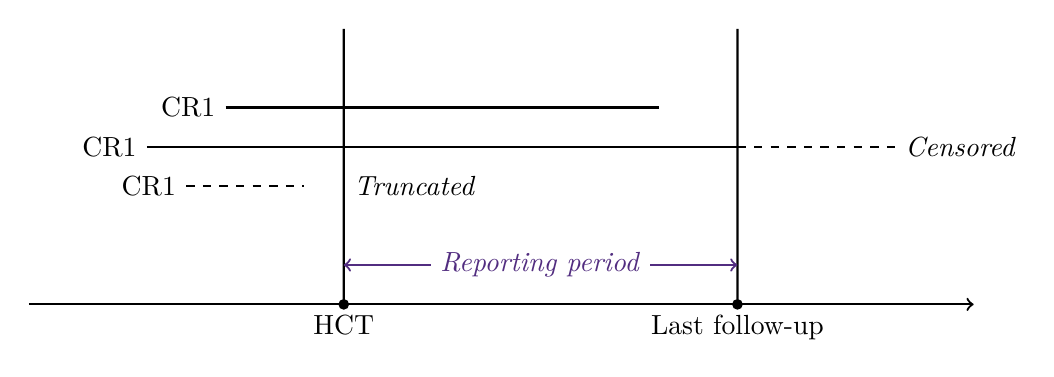
\begin{tikzpicture}[thick, main/.style = {fill = clemsonpurple!15, draw = clemsonpurple, circle}]
      \draw[->] (-4, 0) -- (0, 0) node[below] {HCT} -- (5, 0) node[below] {Last follow-up} -- (8, 0);
      \foreach \x in {0, 5} \draw[fill] (\x, 0) circle (1.5pt) -- (\x, 3.5);
      \draw[<->, clemsonpurple] (0, 0.5) -- (2.5, 0.5) node[fill = white] {\textit{Reporting period}} -- (5, 0.5);

      \draw (-1.5, 2.5) node[left] {CR1} -- (4, 2.5);

      \draw (-2.5, 2) node[left] {CR1} -- (5, 2);
      \draw[dashed] (5, 2) -- (7, 2) node[right] {\textit{Censored}};

      \draw[dashed] (-2, 1.5) node[left] {CR1} -- (-0.5, 1.5) ++(0.5, 0) node[right] {\textit{Truncated}};

    \end{tikzpicture}
  \end{figure}
  The clock starts at CR1 while data is collected at HCT.
  \begin{itemize}
    \item Lifetimes of those who died between HCT and last follow-up are known.
    \item Lifetimes of those who were still alive at last follow-up are particially known (up till the last follow-up).
    \item Lifetimes of those who achieved CR1 with intention to recieve an HCT but did not eventually (e.g., early death) are not observable.
  \end{itemize}
\end{frame}

% \begin{frame}
%   \frametitle{Left truncation - Example}
%   \begin{center}
%     \begin{tikzpicture}[
%       align = center, thick,
%       premain/.style = {draw, minimum size = 10mm},
%       main/.style = {fill = clemsonpurple!15, draw = clemsonpurple, minimum size = 10mm}]
%       \node[premain] (1) {Dx};
%       \node[main] (2) [right = 10mm of 1] {CR1};
%       \node[main] (3) [right = 20mm of 2] {HCT};
%       \node[main] (end1) [right = 25mm of 3] {Death/alive};
%       \draw[->, dashed] (1) -- (2);
%       \draw[->, dashed] (2) -- (3);
%       \draw[->] (3) -- (end1);
%       \node[premain] (4) [below = 5mm of 1] {Dx};
%       \node[main] (5) [right = 20mm of 4] {CR1};
%       \node[main] (6) [right = 10mm of 5] {Chemo};
%       \node[main] (end2) [right = 15mm of 6] {Death/alive};
%       \draw[->] (4) -- (5);
%       \draw[->] (5) -- (6);
%       \draw[->] (6) -- (end2);
%     \end{tikzpicture}
%   \end{center}
%   \begin{itemize}
%     \item The clock starts at CR1.
%     \item Patients who achieved CR1 but did not receive an HCT (e.g., early death) are not observable in the HCT registry.
%   \end{itemize}
% \end{frame}

\begin{frame}
  \frametitle{Adjustment for left-truncated data}
  When calculating number at risk $Y$ at a given time $t$:
  \begin{itemize}
    \item Right censoring:
    \begin{equation*}
      Y = \sum_{i = 1}^n I(T_i \ge t)
    \end{equation*}
    where $T_i$ is the event time of $i$th subject in the sample for $i = 1,\dotsc,n$.
    \item Right censoring and left truncation:
    \begin{equation*}
      Y = \sum_{i = 1}^n I(T_i \ge t > L_i)
    \end{equation*}
    where $T_i$ is the event time and $L_i$ is the truncation/entry time of $i$th subject in the sample for $i = 1,\dotsc,n$.
  \end{itemize}
\end{frame}

\begin{frame}
  \frametitle{Left truncation - Example}
  \begin{columns}
    \begin{column}[]{0.48\textwidth}
      \begin{center}
        \begin{tabular}{c c c}
          $L_i$ & $T_i$ & $\delta_i$ \\\hline
          $1$ & $3$ & $1$ \\
          $1$ & $4$ & $1$ \\
          $2$ & $5$ & $1$ \\
          $4$ & $5$ & $0$ \\
          $4.5$ & $6$ & $1$ \\
          $5.5$ & $6$ & $1$ \\
          $5.6$ & $6$ & $0$ \\
          $2$ & $7$ & $1$ \\
          $3.5$ & $7$ & $1$ \\
          $7.5$ & $9$ & $1$ \\
          $4.5$ & $9$ & $0$ \\\hline
        \end{tabular}
      \end{center}
    \end{column}
    \begin{column}[]{0.48\textwidth}
      \begin{center}
        \begin{tabular}{c c c c}
          $t$ & $d$ & $c$ & $Y$ \\\hline
          $0$ & $0$ & $0$ & $0$ \\
          $3$ & $1$ & $0$ & $4$ \\
          $4$ & $1$ & $0$ & $4$ \\
          $5$ & $1$ & $1$ & $6$ \\
          $6$ & $2$ & $1$ & $6$ \\
          $7$ & $2$ & $0$ & $3$ \\
          $9$ & $1$ & $1$ & $2$ \\\hline
        \end{tabular}
      \end{center}
      \textit{What is the value of $Y$ when $t = 5.5$?}
    \end{column}
  \end{columns}
\end{frame}

\begin{frame}[fragile]
  \frametitle{Left truncation - Example (SAS)}
  \begin{block}{Kaplan-Meier estimator}
    \begin{lstlisting}[gobble = 6]
      proc phreg data = final;
        model indxsurv * dead(0) / entrytime = indxtx;
        baseline out = outsurv survival = _all_ / method = pl;
      run;
    \end{lstlisting}
  \end{block}
  \begin{block}{Cox proportional hazards model}
    \begin{lstlisting}[gobble = 6]
      proc phreg data = final;
        class z1-z10 / ref = first param = ref;
        model indxsurv * dead(0) = z1-z10 / rl entrytime = indxtx;
      run;
    \end{lstlisting}
  \end{block}
  \begin{description}
    \item[\texttt{indxsurv}] Time from diagnosis to death/last follow-up (event time)
    \item[\texttt{indxtx}] Time from diagnosis to transplant (left-truncation time) 
  \end{description}
\end{frame}

\section{Power calculation}

\begin{frame}
  \frametitle{Power calculation and sample size}
  \begin{itemize}
    \item \textbf{Power} Probability that the test correctly rejects the null hypothesis $H_0$ when the alternative hypothesis $H_a$ is true.
    \item Three key components in power calculation:
    \begin{itemize}
      \item Power (usually set at $80\%$)
      \item Sample size
      \item Expected difference in outcomes (based on published literature)
    \end{itemize}
    \item Need two to calculate the third (usually sample size)
  \end{itemize}
\end{frame}

\begin{frame}[fragile]
  \frametitle{Power calculation - Example (SAS)}
  \begin{block}{Code example}
    \begin{lstlisting}[gobble = 6]
      proc power;
        twosamplesurvival
        ntotal = 1861 groupweights = (19 1)
        /* Alternatively: groupns = 1768|93 */
        alpha = .05 sides = 2 test = logrank
        accrualtime = 0.01 followuptime = max
        curve('hct') = (1 to 6 by 1):(0.70 0.59 0.54 0.52 0.50 0.48)
        curve('chemo') = (1 to 3 by 1):(0.79 0.71 0.64)
        groupsurvival = 'hct'|'chemo'
        power = .;
      run;
    \end{lstlisting}
  \end{block}
\end{frame}

\end{document}
